% Created 2019-09-30 Mon 20:09
% Intended LaTeX compiler: pdflatex
\documentclass[11pt]{article}
\usepackage[utf8]{inputenc}
\usepackage[T1]{fontenc}
\usepackage{graphicx}
\usepackage{grffile}
\usepackage{longtable}
\usepackage{wrapfig}
\usepackage{rotating}
\usepackage[normalem]{ulem}
\usepackage{amsmath}
\usepackage{textcomp}
\usepackage{amssymb}
\usepackage{capt-of}
\usepackage{hyperref}
\author{rodri}
\date{\today}
\title{}
\hypersetup{
 pdfauthor={rodri},
 pdftitle={},
 pdfkeywords={},
 pdfsubject={},
 pdfcreator={Emacs 27.0.50 (Org mode 9.2.3)}, 
 pdflang={English}}
\begin{document}

\tableofcontents


\documentclass[12pt,spanish,fleqn,openany,letterpaper,pagesize]{report}

\usepackage[ansinew]{inputenc}
\usepackage[spanish,es-tabla]{babel}
\usepackage{fancyhdr}
\usepackage{epsfig}
\usepackage{epic}
\usepackage{eepic}
\usepackage{amsmath}
\usepackage{threeparttable}
\usepackage{amscd}
\usepackage{here}
\usepackage{graphicx}
\usepackage{lscape}
\usepackage{tabularx}
\usepackage{subfigure}
\usepackage{longtable}
\usepackage{geometry}
\usepackage{pgfplots}

\usepackage{rotating} %Para rotar texto, objetos y tablas seite. No se ve en DVI solo en PS. Seite 328 Hundebuch
                        %se usa junto con \rotate, \sidewidestable ....


\renewcommand{\theequation}{\thechapter-\arabic{equation}}
\renewcommand{\thefigure}{\textbf{\thechapter-\arabic{figure}}}
\renewcommand{\thetable}{\textbf{\thechapter-\arabic{table}}}


\pagestyle{fancyplain}%\addtolength{\headwidth}{\marginparwidth}
\textheight22.5cm \topmargin0cm \textwidth16.5cm
\oddsidemargin0.5cm \evensidemargin-0.5cm%
\renewcommand{\chaptermark}[1]{\markboth{\thechapter\; #1}{}}
\renewcommand{\sectionmark}[1]{\markright{\thesection\; #1}}
\lhead[\fancyplain{}{\thepage}]{\fancyplain{}{\rightmark}}
\rhead[\fancyplain{}{\leftmark}]{\fancyplain{}{\thepage}}
\fancyfoot{}
\thispagestyle{fancy}%


\addtolength{\headwidth}{0cm}
\unitlength1mm %Define la unidad LE para Figuras
\mathindent0cm %Define la distancia de las formulas al texto,  fleqn las descentra
\marginparwidth0cm
\parindent0cm %Define la distancia de la primera linea de un parrafo a la margen

%Para tablas,  redefine el backschlash en tablas donde se define la posici\'{o}n del texto en las
%casillas (con \centering \raggedright o \raggedleft)
\newcommand{\PreserveBackslash}[1]{\let\temp=\\#1\let\\=\temp}
\let\PBS=\PreserveBackslash

%Espacio entre lineas
\renewcommand{\baselinestretch}{1.1}

%Neuer Befehl f\"{u}r die Tabelle Eigenschaften der Aktivkohlen
\newcommand{\arr}[1]{\raisebox{1.5ex}[0cm][0cm]{#1}}

%Neue Kommandos
\usepackage{Befehle}


%Trennungsliste
\hyphenation {Reaktor-ab-me-ssun-gen Gas-zu-sa-mmen-set-zung
Raum-gesch-win-dig-keit Durch-fluss Stick-stoff-gemisch
Ad-sorp-tions-tem-pe-ra-tur Klein-schmidt
Kohlen-stoff-Mole-kular-siebe Py-rolysat-aus-beu-te
Trans-port-vor-gan-ge}
\%\includeonly{Kap1/Kap1,Kap2/Kap2}
\usepackage{titlesec} 
\renewcommand{\tablename}\{\textbf{Tabla}\}
\renewcommand{\figurename}\{\textbf{Figura}\}
\renewcommand{\listtablename}{Lista de Tablas}
\renewcommand{\listfigurename}{Lista de Figuras}
\renewcommand{\labelitemi}{$\bullet$}
\titleformat{\chapter}[display]
\{\bfseries\Large\}
\{\filright\MakeUppercase{\chaptertitlename} \Huge\thechapter\}
\{1ex\}
\{\titlerule\vspace{1ex}\filleft\}
[\vspace{1ex}\titlerule]



\begin{document}

	
\pagenumbering{roman}
%\newpage
%\setcounter{page}{1}
\begin{center}
\begin{figure}
\centering%
\textsc{\large UNIVERSIDAD CAT\'OLICA BOLIVIANA ``SAN PABLO'' }\\[0.3cm] % Name of your university/college
\textsc{\large UNIDAD ACAD\'EMICA REGIONAL LA PAZ}\\[0.3cm] %
\textsc{\large FACULTAD DE INGENIER\'IA}\\[0.3cm]
\textsc{\normalsize  CARRERA DE INGENIER\'IA MECATR\'ONICA}\\[0.1cm]

\epsfig{file=HojaTitulo/UCBSinFondo.png,scale=0.75}%
\end{figure}
\textbf{\large SISTEMA MODULAR DE MEDICIÓN Y GRABADO DIGITAL DE BIO-SEÑALES}\\[0.5cm]

\thispagestyle{empty} \vspace*{0.01cm} \textbf{\large Proyecto de grado presentado para la obtenci\'on del Grado de Ingenier\'ia Mecatr\'onica}\\[0.65cm]

\thispagestyle{empty} \vspace*{0.01cm} \normalsize Por: RODRIGO SEBASTIAN
MENDOZA TEJADA \\[0.8cm]

\thispagestyle{empty} \vspace*{0.01cm} \normalsize Tutor: GUILLERMO SAHONERO ALVAREZ\\[1.5cm]

\vspace*{0.01cm} \normalsize La Paz-Bolivia\\[0.25cm]
\vspace*{0.01cm} \normalsize Noviembre, 2019
\end{center}

\newpage{\pagestyle{empty}\cleardoublepage}

\newpage

\newpage{\pagestyle{empty}\cleardoublepage}

\newpage
\thispagestyle{empty} \textbf{}\normalsize
\\\\\\%
\textbf{DEDICATORIA}\\[4.0cm]

\begin{flushright}
\begin{minipage}{8cm}
    \noindent
        \small
        La dedicatoria es opcional y cada autor podr\'a determinar la distribuci\'on del texto en la p\'{a}gina, se sugiere esta presentaci\'on. En ella el autor dedica su trabajo en forma especial a personas y/o entidades.\\[1.0cm]\\
        Por ejemplo:\\[1.0cm]
        A mis padres\\[1.0cm]\\
        o\\[1.0cm]
        La preocupaci\'on por el hombre y su destino siempre debe ser el
        inter\'es primordial de todo esfuerzo t\'ecnico. Nunca olvides esto
        entre tus diagramas y ecuaciones.\\\\
        Albert Einstein\\
\end{minipage}
\end{flushright}

%\newpage{\pagestyle{empty}\cleardoublepage}

\newpage
\thispagestyle{empty} \textbf{}\normalsize
\\\\\\%
\textbf{AGRADECIMIENTOS}
%\addcontentsline{toc}{chapter}{\numberline{}Agradecimientos}\\\\
\\\\
Esta secci\'{o}n es opcional, en ella el autor agradece a las personas o instituciones que colaboraron en la realizaci\'{o}n de la tesis  o trabajo de investigaci\'{o}n. Si se incluye esta secci\'{o}n, deben aparecer los nombres completos, los cargos y su aporte al documento.\\

\newpage{\pagestyle{empty}\cleardoublepage}

\newpage
\textbf{\LARGE Resumen}\\\\
%\addcontentsline{toc}{chapter}{\numberline{}Resumen}
\\\\
El resumen es una presentaci\'{o}n abreviada y precisa (la NTC 1486 de 2008 recomienda revisar la norma ISO 214 de 1976). Se debe usar una extensi\'{o}n m\'{a}xima de 15 renglones. Se recomienda que este resumen sea anal\'{\i}tico, es decir, que sea completo, con informaci\'{o}n cuantitativa y cualitativa, generalmente incluyendo los siguientes aspectos: objetivos, dise\~{n}o, lugar y circunstancias, objetivo del estudio, intervenci\'{o}n, mediciones y principales resultados, y conclusiones. Al final del resumen se deben usar palabras claves tomadas del texto (m\'{\i}nimo 3 y m\'{a}ximo 7 palabras), las cuales permiten la recuperaci\'{o}n de la informaci\'{o}n.\\

\textbf{\small \textit{Palabras clave: (m\'{a}ximo 10 palabras, preferiblemente seleccionadas de las listas internacionales que permitan el indizado cruzado)}}.\\

\textbf{\small L\'inea de investigaci\'on:} \small (m\'aximo 1 o 2  rengl\'ones en que se establezca la  l\'inea de investigaci\'on a la que pertenece el proyecto de grado).\\


\newpage
\textbf{\LARGE Abstract}\\\\
Es el mismo resumen pero traducido al ingl\'{e}s. Se debe usar una extensi\'{o}n m\'{a}xima de 12 renglones. Al final del Abstract se deben traducir las anteriores palabras claves tomadas del texto (m\'{\i}nimo 3 y m\'{a}ximo 7 palabras), llamadas keywords. Es posible incluir el resumen en otro idioma diferente al espa\~{n}ol o al ingl\'{e}s, si se considera como importante dentro del tema tratado en la investigaci\'{o}n, por ejemplo: un trabajo dedicado a problemas ling\"{u}\'{\i}sticos del mandar\'{\i}n seguramente estar\'{\i}a mejor con un resumen en mandar\'{\i}n.\\[2.0cm]
\textbf{\small \textit {Keywords: palabras clave en ingl\'es(m\'aximo 10 palabras, preferiblemente seleccionadas de las listas internacionales que permitan el indizado cruzado)}}\\

\textbf{\small Research area:} \small texto en ingl\'es (m\'aximo 1 o 2  rengl\'ones en que se establezca la  l\'inea de investigaci\'on a la que pertenece el proyecto de grado).\\

\renewcommand{\contentsname}{\textbf{\LARGE \'Indice}}


%\chapter*{Lista de s\'imbolos}
%\textbf{\Large Lista de s\'imbolos} \\\\
\textbf{\LARGE Notaci\'on}\\\\
%\lhead{\emph{Lista de s\'imbolos}}
%\addcontentsline{toc}{chapter}{\numberline{}Lista de s\'{\i}mbolos}
Esta secci\'{o}n es opcional, dado que existen disciplinas que no manejan s\'{\i}mbolos y/o abreviaturas.\\

Se incluyen s\'{\i}mbolos generales (con letras latinas y griegas), sub\'{\i}ndices, super\'{\i}ndices y abreviaturas (incluir s\'{o}lo las clases de s\'{\i}mbolos que se utilicen). Cada una de estas listas debe estar ubicada en orden alfab\'{e}tico de acuerdo con la primera letra del s\'{\i}mbolo.
%\section*{S\'{\i}mbolos con letras latinas}
 \label{simbolos}
 \renewcommand{\arraystretch}{1.3}
%\begin{longtable}[l]{*{4}{>{$}l<{$}}p{9cm}}
%\begin{longtable}[l]{>{$}l<{$}l>{$}l<{$}>{$}l<{$}}
\begin{longtable}[l]{>{$}l<{$}l>{$}l<{$}}
%\begin{tabular}
\textbf{S\'{\i}mbolo}&\textbf{T\'{e}rmino}&\\[0.6ex]\hline
\endfirsthead%
\textbf{S\'{\i}mbolo}&\textbf{T\'{e}rmino}&\\[0.6ex]\hline
\endhead%
      I_{\text{max}}        & Corriente m\'axima[\textit A]                                                  \\%
      \alpha &tasa de aprendizaje                     \\%
      \lambda_{\text{i}}   & Autovalor i                             \\%

\end{longtable}
\vspace{5ex}



\section*{Glosario}
\begin{longtable}[l]{>{}l<{}l}
  \textbf{Abreviatura} & \textbf{T\'{e}rmino} \\[0.5ex] \hline%
  \endfirsthead%
  \textbf{Abreviatura} & \textbf{T\'{e}rmino} \\[0.5ex] \hline%
  \endhead%
\renewcommand{\arraystretch}{1.4}\label{simbolosg}
 $DP$&Deep Learning - Aprendizaje profundo \\%
 $FCEM$    & Fuerza contraelectromotriz\\%
 $RAM$   &Random Access Memory - Memoria de Acceso Aleatorio\\%

\end{longtable}


\setlength{\extrarowheight}{0pt}
%\newcommand{\clearemptydoublepage}{\newpage{\pagestyle{empty}\cleardoublepage}}

\tableofcontents
\listoffigures

\listoftables
%\include{Resumen}%\newcommand{\clearemptydoublepage}{\newpage{\pagestyle{empty}\cleardoublepage}}
\newpage
\pagenumbering{arabic}


\chapter{Marco Referencial}
\section{Introducci\'on}

En la introducci\'{o}n, el autor presenta y se\~{n}ala la importancia, el origen (los antecedentes te\'{o}ricos y pr\'{a}cticos), los objetivos, los alcances, las limitaciones, la metodolog\'{\i}a empleada, el significado que el estudio tiene en el avance del campo respectivo y su aplicaci\'{o}n en el \'{a}rea investigada. No debe confundirse con el resumen y se recomienda que la introducci\'{o}n tenga una extensi\'{o}n de m\'{\i}nimo 2 p\'{a}ginas y m\'{a}ximo de 4 p\'{a}ginas.\\

La presente plantilla maneja una familia de fuentes utilizada generalmente en LaTeX, conocida como Computer Modern, espec\'{\i}ficamente LMRomanM para el texto de los p\'{a}rrafos y CMU Sans Serif para los t\'{\i}tulos y subt\'{\i}tulos. Sin embargo, es posible sugerir otras fuentes tales como Garomond, Calibri, Cambria, Arial o Times New Roman, que por claridad y forma, son adecuadas para la edici\'{o}n de textos acad\'{e}micos.\\

La presente plantilla tiene en cuenta aspectos importantes de la Norma T\'{e}cnica Colombiana - NTC 1486, con el fin que sea usada para la presentaci\'{o}n final de las tesis de maestr\'{\i}a y doctorado y especializaciones y especialidades en el \'{a}rea de la salud, desarrolladas en la Universidad Nacional de Colombia.\\

Las m\'{a}rgenes, numeraci\'{o}n, tama\~{n}o de las fuentes y dem\'{a}s aspectos de formato, deben ser conservada de acuerdo con esta plantilla, la cual esta dise\~{n}ada para imprimir por lado y lado en hojas tama\~{n}o carta. Se sugiere que los encabezados cambien seg\'{u}n la secci\'{o}n del documento (para lo cual esta plantilla esta construida por secciones).\\

Si se requiere ampliar la informaci\'{o}n sobre normas adicionales para la escritura se puede consultar la norma NTC 1486 en la Base de datos del ICONTEC (Normas T\'{e}cnicas Colombianas) disponible en el portal del SINAB de la Universidad Nacional de Colombia\footnote{ver: www.sinab.unal.edu.co}, en la secci\'{o}n "Recursos bibliogr\'{a}ficos" opci\'{o}n "Bases de datos".  Este portal tambi\'{e}n brinda la posibilidad de acceder a un instructivo para la utilizaci\'{o}n de Microsoft Word y Acrobat Professional, el cual est\'{a} disponible en la secci\'{o}n "Servicios", opci\'{o}n "Tr\'{a}mites" y enlace "Entrega de tesis".\\

La redacci\'{o}n debe ser impersonal y gen\'{e}rica. La numeraci\'{o}n de las hojas sugiere que las p\'{a}ginas preliminares se realicen en n\'{u}meros romanos en may\'{u}scula y las dem\'{a}s en n\'{u}meros ar\'{a}bigos, en forma consecutiva a partir de la introducci\'{o}n que comenzar\'{a} con el n\'{u}mero 1. La cubierta y la portada no se numeran pero si se cuentan como p\'{a}ginas.\\

Para trabajos muy extensos se recomienda publicar m\'{a}s de un volumen. Se debe tener en cuenta que algunas facultades tienen reglamentada la extensi\'{o}n m\'{a}xima de las tesis  o trabajo de investigaci\'{o}n; en caso que no sea as\'{\i}, se sugiere que el documento no supere 120 p\'{a}ginas.\\

No se debe utilizar numeraci\'{o}n compuesta como 13A, 14B \'{o} 17 bis, entre otros, que indican superposici\'{o}n de texto en el documento. Para resaltar, puede usarse letra cursiva o negrilla. Los t\'{e}rminos de otras lenguas que aparezcan dentro del texto se escriben en cursiva.\\

\section{Planteamiento del Problema}
\subsection{Definici\'on del problema}

\section{Objetivos}
\subsection{Objetivo General}
\subsection{Objetivos espec\'ificos}
\begin{itemize}
	
	\item Objetivo espec\'ifico 1 
	\item Objetivo espec\'ifico 2 
	\item Objetivo espec\'ifico 3 
	\item Objetivo espec\'ifico 4 
	\item Objetivo espec\'ifico 5 
	\item Objetivo espec\'ifico 6 
\end{itemize}


\section{Justificaci\'on}
\section{L\'imites y Alcances}
\subsection{L\'imites}
\begin{itemize}
	
	\item L\'imite 1 
	\item L\'imite 2 
	\item L\'imite 3 
	\item L\'imite 4 
	\item L\'imite 5 
	\item L\'imiteo 6 
\end{itemize}
\subsection{Alcances}

\begin{itemize}
	
	\item Alcance 1 
	\item Alcance 2
	\item Alcance 3
	\item Alcance 4
	\item Alcance 5
	\item Alcance 6
\end{itemize}

\chapter{Marco Te\'orico}
Los cap\'{\i}tulos son las principales divisiones del documento. En estos, se desarrolla el tema del documento. Cada cap\'{\i}tulo debe corresponder a uno de los temas o aspectos tratados en el documento y por tanto debe llevar un t\'{\i}tulo que indique el contenido del cap\'{\i}tulo.\\

Los t\'{\i}tulos de los cap\'{\i}tulos deben ser concertados entre el alumno y el director de la tesis  o trabajo de investigaci\'{o}n, teniendo en cuenta los lineamientos que cada unidad acad\'{e}mica brinda. As\'{\i} por ejemplo, en algunas facultades se especifica que cada cap\'{\i}tulo debe corresponder a un art\'{\i}culo cient\'{\i}fico, de tal manera que se pueda publicar posteriormente en una revista.\\

\section{Estado del Arte}
Es evidenete que esta secci\'on trata de una extensa revisi\'on bibliogr\'afica, por lo que se deber\'a referenciar una cantidad importante de papers. 

Existen varias normas para la citaci\'{o}n bibliogr\'{a}fica. Algunas \'{a}reas del conocimiento prefieren normas espec\'{\i}ficas para citar las referencias bibliogr\'{a}ficas en el texto y escribir la lista de bibliograf\'{\i}a al final de los documentos. Esta plantilla brinda la libertad para que el autor de la tesis  o trabajo de investigaci\'{o}n utilice la norma bibliogr\'{a}fica com\'{u}n para su disciplina. Sin embargo, se solicita que la norma seleccionada se utilice con rigurosidad, sin olvidar referenciar "todos" los elementos tomados de otras fuentes (referencias bibliogr\'{a}ficas, patentes consultadas, software empleado en el manuscrito, en el tratamiento a los datos y resultados del trabajo, consultas a personas (expertos o p\'{u}blico general), entre otros).\\

Existen algunos ejemplos para la citaci\'{o}n bibliogr\'{a}fica, por ejemplo, Microsoft Word (versiones posteriores al 2006), en el  men\'{u} de referencias, se cuenta con la opci\'{o}n de insertar citas bibliogr\'{a}ficas utilizando la norma APA (American Psychological Association) u otras normas y con la ayuda para construir autom\'{a}ticamente la lista al final del documento. De la misma manera, existen administradores bibliogr\'{a}ficos compatibles con Microsoft Word como Zotero, End Note y el Reference Manager,  disponibles a trav\'{e}s del Sistema Nacional de Bibliotecas (SINAB) de la Universidad Nacional de Colombia\footnote{Ver:www.sinab.unal.edu.co } secci\'{o}n "Recursos bibliogr\'{a}ficos" opci\'{o}n "Herramientas Bibliogr\'{a}ficas. A continuaci\'{o}n se muestra un ejemplo de una de las formas m\'{a}s usadas para las citaciones bibliogr\'{a}ficas.\\

Citaci\'{o}n individual:\cite{AG01}.\\
Citaci\'{o}n simult\'{a}nea de varios autores:
\cite{AG12,AG52,AG70,AG08a,AG09a,AG36a,AG01i}.\\

Por lo general, las referencias bibliogr\'{a}ficas correspondientes a los anteriores n\'{u}meros, se listan al final del documento en orden de aparici\'{o}n o en orden alfab\'{e}tico. Otras normas de citaci\'{o}n incluyen el apellido del autor y el a\~{n}o de la referencia, por ejemplo: 1) "...\'{e}nfasis en elementos ligados al \'{a}mbito ingenieril que se enfocan en el manejo de datos e informaci\'{o}n estructurada y que seg\'{u}n Kostoff (1997) ha atra\'{\i}do la atenci\'{o}n de investigadores dado el advenimiento de TIC...", 2) "...Dicha afirmaci\'{o}n coincide con los planteamientos de Snarch (1998), citado por Castellanos (2007), quien comenta que el manejo..." y 3) "...el futuro del sistema para argumentar los procesos de toma de decisiones y el desarrollo de ideas innovadoras (Nosella \textsl{et al}., 2008)...".\\

\subsection{Enfoque 1}
De la cuarta subdivisi\'{o}n en adelante, cada nueva divisi\'{o}n o \'{\i}tem puede ser se\~{n}alada con vi\~{n}etas, conservando el mismo estilo de \'{e}sta, a lo largo de todo el documento.\\

Las subdivisiones, las vi\~{n}etas y sus textos acompa\~{n}antes deben presentarse sin sangr\'{\i}a y justificados.\\

\subsection{Enfoque 2}
De la cuarta subdivisi\'{o}n en adelante, cada nueva divisi\'{o}n o \'{\i}tem puede ser se\~{n}alada con vi\~{n}etas, conservando el mismo estilo de \'{e}sta, a lo largo de todo el documento.\\
\subsection{Enfoque n}
De la cuarta subdivisi\'{o}n en adelante, cada nueva divisi\'{o}n o \'{\i}tem puede ser se\~{n}alada con vi\~{n}etas, conservando el mismo estilo de \'{e}sta, a lo largo de todo el documento.\\

\subsection{Discusi\'on}
De la cuarta subdivisi\'{o}n en adelante, cada nueva divisi\'{o}n o \'{\i}tem puede ser se\~{n}alada con vi\~{n}etas, conservando el mismo estilo de \'{e}sta, a lo largo de todo el documento.\\

Es recomendable incluir una tabla resumen de comparaci\'on entre las diferentes soluciones.

Para la edici\'{o}n de tablas, cada columna debe llevar su t\'{\i}tulo; la primera palabra se debe escribir con may\'{u}scula inicial y preferiblemente sin abreviaturas. En las tablas y cuadros, los t\'{\i}tulos y datos se deben ubicar entre l\'{\i}neas horizontales y verticales cerradas (como se realiza en esta plantilla).\\

La numeraci\'{o}n de las tablas se realiza de la misma manera que las figuras o ilustraciones, a lo largo de todo el texto. Deben llevar un t\'{\i}tulo breve, que concreta el contenido de la tabla; \'{e}ste se debe escribir en la parte superior de la misma. Para la presentaci\'{o}n de cuadros, se deben seguir las indicaciones dadas para las tablas.\\

Un ejemplo para la presentaci\'{o}n y citaci\'{o}n de tablas (citaci\'{o}n indirecta), se presenta a continuaci\'{o}n:\\

\begin{center}
	\begin{threeparttable}
		\centering%
		\caption{Participaci\'{o}n de las energ\'{\i}as renovables en el suministro
			total de energ\'{\i}a primaria \cite{AG02i}.}\label{EMundo1}
		\begin{tabular}{|l|c|c|}\hline
			&\multicolumn{2}{c|}{Participaci\'{o}n en el suministro de energ\'{\i}a primaria /\% (Mtoe)\;$\tnote{1}$}\\\cline{2-3}%
			\arr{Region}&Energ\'{\i}as renovables &Participaci\'{o}n de la biomasa\\\hline%
			Latinoam\'{e}rica&28,9 (140)&62,4 (87,4)\\\hline%
			\:Colombia&27,7 (7,6)&54,4 (4,1)\\\hline%
			Alemania&3,8 (13,2)&65,8 (8,7)\\\hline%
			Mundial&13,1 (1404,0)&79,4 (1114,8)\\\hline
		\end{tabular}
		\begin{tablenotes}
			\item[1] \footnotesize{1 kg oe=10000 kcal=41,868 MJ}
		\end{tablenotes}
	\end{threeparttable}
\end{center}

\section{Fundamentos Te\'oricos}
\subsection{T\'ecnica/concepto/Algoritmo 1}
Recuerde incluir la ecuaciones debidas como se muestra a continuaci\'on:
	\begin{equation}\label{fuerza}
	F = ma
	\end{equation}
Donde: \\ 
\(F\) es fuerza\\
\(m\) es masa\\
\(a\) es aceleraci\'on\\
La ecuaci\'on  \ref{fuerza} es utilizada para determinar la .... 

\subsection{T\'ecnica/concepto/Algoritmo 2}
\subsection{T\'ecnica/concepto/Algoritmo 3}
\subsection{T\'ecnica/concepto/Algoritmo n}


\chapter{Marco Pr\'actico}
Texto introductorio de lo que se desarollar\'a en este cap\'itulo.\\

\section{Esquema general del proyecto}
Existen algunos ejemplos para la citaci\'{o}n bibliogr\'{a}fica, por ejemplo, Microsoft Word (versiones posteriores al 2006), en el  men\'{u} de referencias, se cuenta con la opci\'{o}n de insertar citas bibliogr\'{a}ficas utilizando la norma APA (American Psychological Association) u otras normas y con la ayuda para construir autom\'{a}ticamente la lista al final del documento. De la misma manera, existen administradores bibliogr\'{a}ficos compatibles con Microsoft Word como Zotero, End Note y el Reference Manager,  disponibles a trav\'{e}s del Sistema Nacional de Bibliotecas (SINAB) de la Universidad Nacional de Colombia\footnote{Ver:www.sinab.unal.edu.co } secci\'{o}n "Recursos bibliogr\'{a}ficos" opci\'{o}n "Herramientas Bibliogr\'{a}ficas. A continuaci\'{o}n se muestra un ejemplo de una de las formas m\'{a}s usadas para las citaciones bibliogr\'{a}ficas.\\

Citaci\'{o}n individual:\cite{AG01}.\\
Citaci\'{o}n simult\'{a}nea de varios autores:
\cite{AG12,AG52,AG70,AG08a,AG09a,AG36a,AG01i}.\\

Por lo general, las referencias bibliogr\'{a}ficas correspondientes a los anteriores n\'{u}meros, se listan al final del documento en orden de aparici\'{o}n o en orden alfab\'{e}tico. Otras normas de citaci\'{o}n incluyen el apellido del autor y el a\~{n}o de la referencia, por ejemplo: 1) "...\'{e}nfasis en elementos ligados al \'{a}mbito ingenieril que se enfocan en el manejo de datos e informaci\'{o}n estructurada y que seg\'{u}n Kostoff (1997) ha atra\'{\i}do la atenci\'{o}n de investigadores dado el advenimiento de TIC...", 2) "...Dicha afirmaci\'{o}n coincide con los planteamientos de Snarch (1998), citado por Castellanos (2007), quien comenta que el manejo..." y 3) "...el futuro del sistema para argumentar los procesos de toma de decisiones y el desarrollo de ideas innovadoras (Nosella \textsl{et al}., 2008)...".\\

\section{Etapa 1}


Al realizarse la ingenier\'ia del proyecto, es com\'un que sea necesario incluir im\'agenes de evidencien el desarrollo del proyecto. 
Las ilustraciones forman parte del contenido de los cap\'{\i}tulos. Se deben colocar en la misma p\'{a}gina en que se mencionan o en la siguiente (deben siempre mencionarse en el texto).\\

\subsection{Requerimientos}

Las llamadas para explicar alg\'{u}n aspecto de la informaci\'{o}n deben hacerse con nota al pie y su nota correspondiente\footnote{Las notas van como "notas al pie". Se utilizan para explicar, comentar o hacer referencia al texto de un documento, as\'{\i} como para introducir comentarios detallados y en ocasiones para citar fuentes de informaci\'{o}n (aunque para esta opci\'{o}n es mejor seguir en detalle las normas de citaci\'{o}n bibliogr\'{a}fica seleccionadas).}. La fuente documental se debe escribir al final de la ilustraci\'{o}n o figura con los elementos de la referencia (de acuerdo con las normas seleccionadas) y no como pie de p\'{a}gina. Un ejemplo para la presentaci\'{o}n y citaci\'{o}n de figuras, se presenta a continuaci\'{o}n (citaci\'{o}n directa):\\

\subsection{C\'alculos/dimensionamiento}

\subsection{Desarrollo }
Por medio de las propiedades del fruto, seg\'{u}n el espesor del endocarpio, se hace una clasificaci\'{o}n de la palma de aceite en tres tipos: Dura, Ternera y Pisifera, que se ilustran en la Figura
\ref{fig:Fruto}.\\
\begin{figure}
\centering%
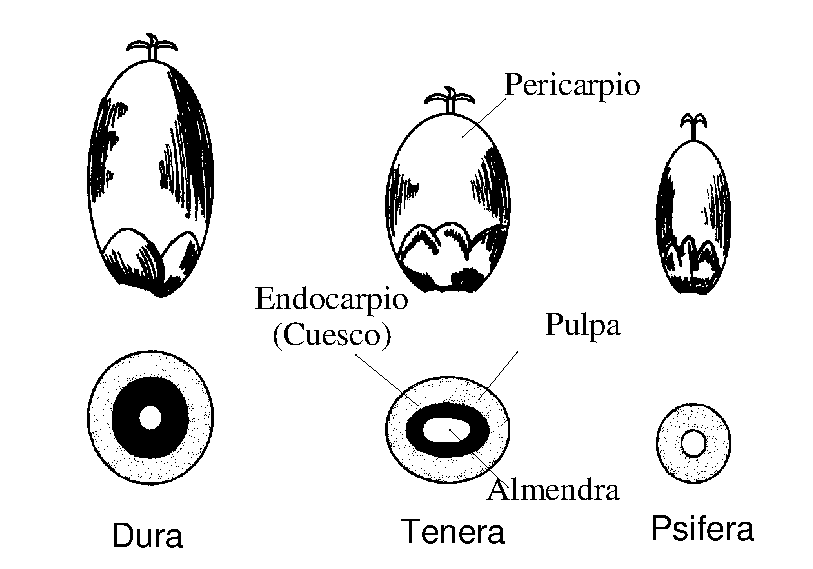
\includegraphics{Kap3/FrutoSp}%
\caption{Tipos y partes del fruto de palma de aceite \cite{AG03p,AG04p}.} \label{fig:Fruto}
\end{figure}

\section{Etapa 2}
Para la edici\'{o}n de tablas, cada columna debe llevar su t\'{\i}tulo; la primera palabra se debe escribir con may\'{u}scula inicial y preferiblemente sin abreviaturas. En las tablas y cuadros, los t\'{\i}tulos y datos se deben ubicar entre l\'{\i}neas horizontales y verticales cerradas (como se realiza en esta plantilla).\\

\subsection{Requerimientos}


\subsection{C\'alculos/dimensionamiento}

\subsection{Desarrollo }
La numeraci\'{o}n de las tablas se realiza de la misma manera que las figuras o ilustraciones, a lo largo de todo el texto. Deben llevar un t\'{\i}tulo breve, que concreta el contenido de la tabla; \'{e}ste se debe escribir en la parte superior de la misma. Para la presentaci\'{o}n de cuadros, se deben seguir las indicaciones dadas para las tablas.\\

Un ejemplo para la presentaci\'{o}n y citaci\'{o}n de tablas (citaci\'{o}n indirecta), se presenta a continuaci\'{o}n:\\

De esta participaci\'{o}n aproximadamente el 60 \% proviene de biomasa
(Tabla \ref{EMundo1}).
\begin{center}
\begin{threeparttable}
\centering%
\caption{Participaci\'{o}n de las energ\'{\i}as renovables en el suministro
total de energ\'{\i}a primaria \cite{AG02i}.}\label{EMundo1}
\begin{tabular}{|l|c|c|}\hline
&\multicolumn{2}{c|}{Participaci\'{o}n en el suministro de energ\'{\i}a primaria /\% (Mtoe)\;$\tnote{1}$}\\\cline{2-3}%
\arr{Region}&Energ\'{\i}as renovables &Participaci\'{o}n de la biomasa\\\hline%
Latinoam\'{e}rica&28,9 (140)&62,4 (87,4)\\\hline%
\:Colombia&27,7 (7,6)&54,4 (4,1)\\\hline%
Alemania&3,8 (13,2)&65,8 (8,7)\\\hline%
Mundial&13,1 (1404,0)&79,4 (1114,8)\\\hline
\end{tabular}
\begin{tablenotes}
\item[1] \footnotesize{1 kg oe=10000 kcal=41,868 MJ}
\end{tablenotes}
\end{threeparttable}
\end{center}

NOTA: en el caso en que el contenido de la tabla o cuadro sea muy extenso, se puede cambiar el tama\~{n}o de la letra, siempre y cuando \'{e}sta sea visible por el lector.\\

\section{Etapa 3}
\subsection{Requerimientos}
\subsection{C\'alculos/dimensionamiento}

\subsection{Desarrollo }

\section{Herramientas}

\subsection{Hardware}
\subsection{Software}

\section{Resultados y discusi\'on}




\chapter{Marco Conclusivo}
\section{Conclusiones}
Las conclusiones constituyen un cap\'{\i}tulo independiente y presentan, en forma l\'{o}gica, los resultados de la tesis  o trabajo de investigaci\'{o}n. Las conclusiones deben ser la respuesta a los objetivos o prop\'{o}sitos planteados. Se deben titular con la palabra conclusiones en el mismo formato de los t\'{\i}tulos de los cap\'{\i}tulos anteriores (T\'{\i}tulos primer nivel), precedida por el numeral correspondiente (seg\'{u}n la presente plantilla).\\

\section{Recomendaciones}
Se presentan como una serie de aspectos que se podr\'{\i}an realizar en un futuro para emprender investigaciones similares o fortalecer la investigaci\'{o}n realizada. Deben contemplar las perspectivas de la investigaci\'{o}n, las cuales son sugerencias, proyecciones o alternativas que se presentan para modificar, cambiar o incidir sobre una situaci\'{o}n espec\'{\i}fica o una problem\'{a}tica encontrada. Pueden presentarse como un texto con caracter\'{\i}sticas argumentativas, resultado de una reflexi\'{o}n acerca de la tesis o trabajo de investigaci\'{o}n.\\

\section{Trabajo Futuro}

\addcontentsline{toc}{chapter}{\numberline{}Bibliograf\'{\i}a}
\bibliographystyle{plaindin_esp}
\bibliography{BibliMSc}
\begin{appendix}
\chapter{Anexo: Nombrar el anexo A de acuerdo con su contenido}\label{AnexoA}
Los Anexos son documentos o elementos que complementan el cuerpo de la tesis o trabajo de investigaci\'{o}n y que se relacionan, directa o indirectamente, con la investigaci\'{o}n, tales como acetatos, cd, normas, etc.\\

\chapter{Anexo: Nombrar el anexo B de acuerdo con su contenido}
A final del documento es opcional incluir \'{\i}ndices o glosarios. \'{E}stos son listas detalladas y especializadas de los t\'{e}rminos, nombres, autores, temas, etc., que aparecen en el mismo. Sirven para facilitar su localizaci\'{o}n en el texto. Los \'{\i}ndices pueden ser alfab\'{e}ticos, cronol\'{o}gicos, num\'{e}ricos, anal\'{\i}ticos, entre otros. Luego de cada palabra, t\'{e}rmino, etc., se pone coma y el n\'{u}mero de la p\'{a}gina donde aparece esta informaci\'{o}n.\\

\chapter{Anexo: Nombrar el anexo C de acuerdo con su contenido}
MANEJO DE LA BIBLIOGRAF\'{I}A: la bibliograf\'{\i}a es la relaci\'{o}n de las fuentes documentales consultadas por el investigador para sustentar sus trabajos. Su inclusi\'{o}n es obligatoria en todo trabajo de investigaci\'{o}n. Cada referencia bibliogr\'{a}fica se inicia contra el margen izquierdo.\\

La NTC 5613 establece los requisitos para la presentaci\'{o}n de referencias bibliogr\'{a}ficas citas y notas de pie de p\'{a}gina. Sin embargo, se tiene la libertad de usar cualquier norma bibliogr\'{a}fica de acuerdo con lo acostumbrado por cada disciplina del conocimiento. En esta medida es necesario que la norma seleccionada se aplique con rigurosidad.\\

Es necesario tener en cuenta que la norma ISO 690:1987 (en Espa\~{n}a, UNE 50-104-94) es el marco internacional que da las pautas m\'{\i}nimas para las citas bibliogr\'{a}ficas de documentos impresos y publicados. A continuaci\'{o}n se lista algunas instituciones que brindan par\'{a}metros para el manejo de las referencias bibliogr\'{a}ficas:\\

\begin{center}
\centering%
\begin{tabular}{|p {7.5 cm}|p {7.5 cm}|}\hline
\arr{Instituci\'{o}n}&Disciplina de aplicaci\'{o}n\\\hline%
Modern Language Association (MLA)&Literatura, artes y humanidades\\\hline%
American Psychological Association (APA)&Ambito de la salud (psicolog\'{\i}a, medicina) y en general en todas las ciencias sociales\\\hline
Universidad de Chicago/Turabian &Periodismo, historia y humanidades.\\\hline
AMA (Asociaci\'{o}n M\'{e}dica de los Estados Unidos)&Ambito de la salud (psicolog\'{\i}a, medicina)\\\hline
Vancouver &Todas las disciplinas\\\hline
Council of Science Editors (CSE)&En la actualidad abarca diversas ciencias\\\hline
National Library of Medicine (NLM) (Biblioteca Nacional de Medicina)&En el \'{a}mbito m\'{e}dico y, por extensi\'{o}n, en ciencias.\\\hline
Harvard System of Referencing Guide &Todas las disciplinas\\\hline
JabRef y KBibTeX &Todas las disciplinas\\\hline
\end{tabular}
\end{center}

Para incluir las referencias dentro del texto y realizar lista de la bibliograf\'{\i}a en la respectiva secci\'{o}n, puede utilizar las herramientas que Latex suministra o, revisar el instructivo desarrollado por el Sistema de Bibliotecas de la Universidad Nacional de Colombia\footnote{Ver: www.sinab.unal.edu.co}, disponible en la secci\'{o}n "Servicios", opci\'{o}n "Tr\'{a}mites" y enlace "Entrega de tesis".

\end{appendix}

\end{document}
\section{Marco Referencial}
\label{sec:org837fd35}
\section{Marco teórico}
\label{sec:org45e9a7d}
\subsection{Estado del arte [obj especificos]}
\label{sec:org7233cea}
\subsubsection{Neurosky}
\label{sec:org55318ff}
\subsubsection{Tecnico}
\label{sec:org776a278}
\subsubsection{Modular}
\label{sec:org59cc94e}
\subsection{Fundamentos}
\label{sec:orge32a7ca}
\subsubsection{siencia investigada para desarrollar}
\label{sec:org3c1f3d6}
\subsubsection{ADCS}
\label{sec:orge26b4c3}
\subsubsection{Impedancia - aplicado}
\label{sec:org16e3c2a}
\subsubsection{NO EXPLICAR Q ES BODE}
\label{sec:org66d30c1}
\subsubsection{EXPLICAR ANCHO DE BANDA}
\label{sec:org661008c}
\end{document}